\chapter{آزمایش و نتایج}
\section{ساختار نرم‌افزاری \lr{Kompute}}
به منظور تست الگوریتمی که در بخش پیشین ارائه گردید، یک ساختار نرم‌افزاری (فریم‌ورک) با نام \lr{Kompute} در زبان \lr{Kotlin} تعبیه شده است. با استفاده از این فریم‌ورک می‌توان الگوریتم جستجوی استراتژی تخلیه بهینه را به ازای پارامترهای محیطی مختلف اجرا کرد و عملکرد استراتژی بدست آمده از الگوریتم را با کمک شبیه‌سازی با سایر استراتژی‌ها مقایسه کرد. این فریم‌ورک طبق یافته‌های ما اولین پیاده‌سازی متن‌باز در زمینه استراتژی تخلیه وظایف ناهمگون است. \\

معماری کلی این فریم‌ورک در قالب یک کلاس دیاگرام در صفحه بعد آورده شده است.
\newpage
\begin{figure}[H]
	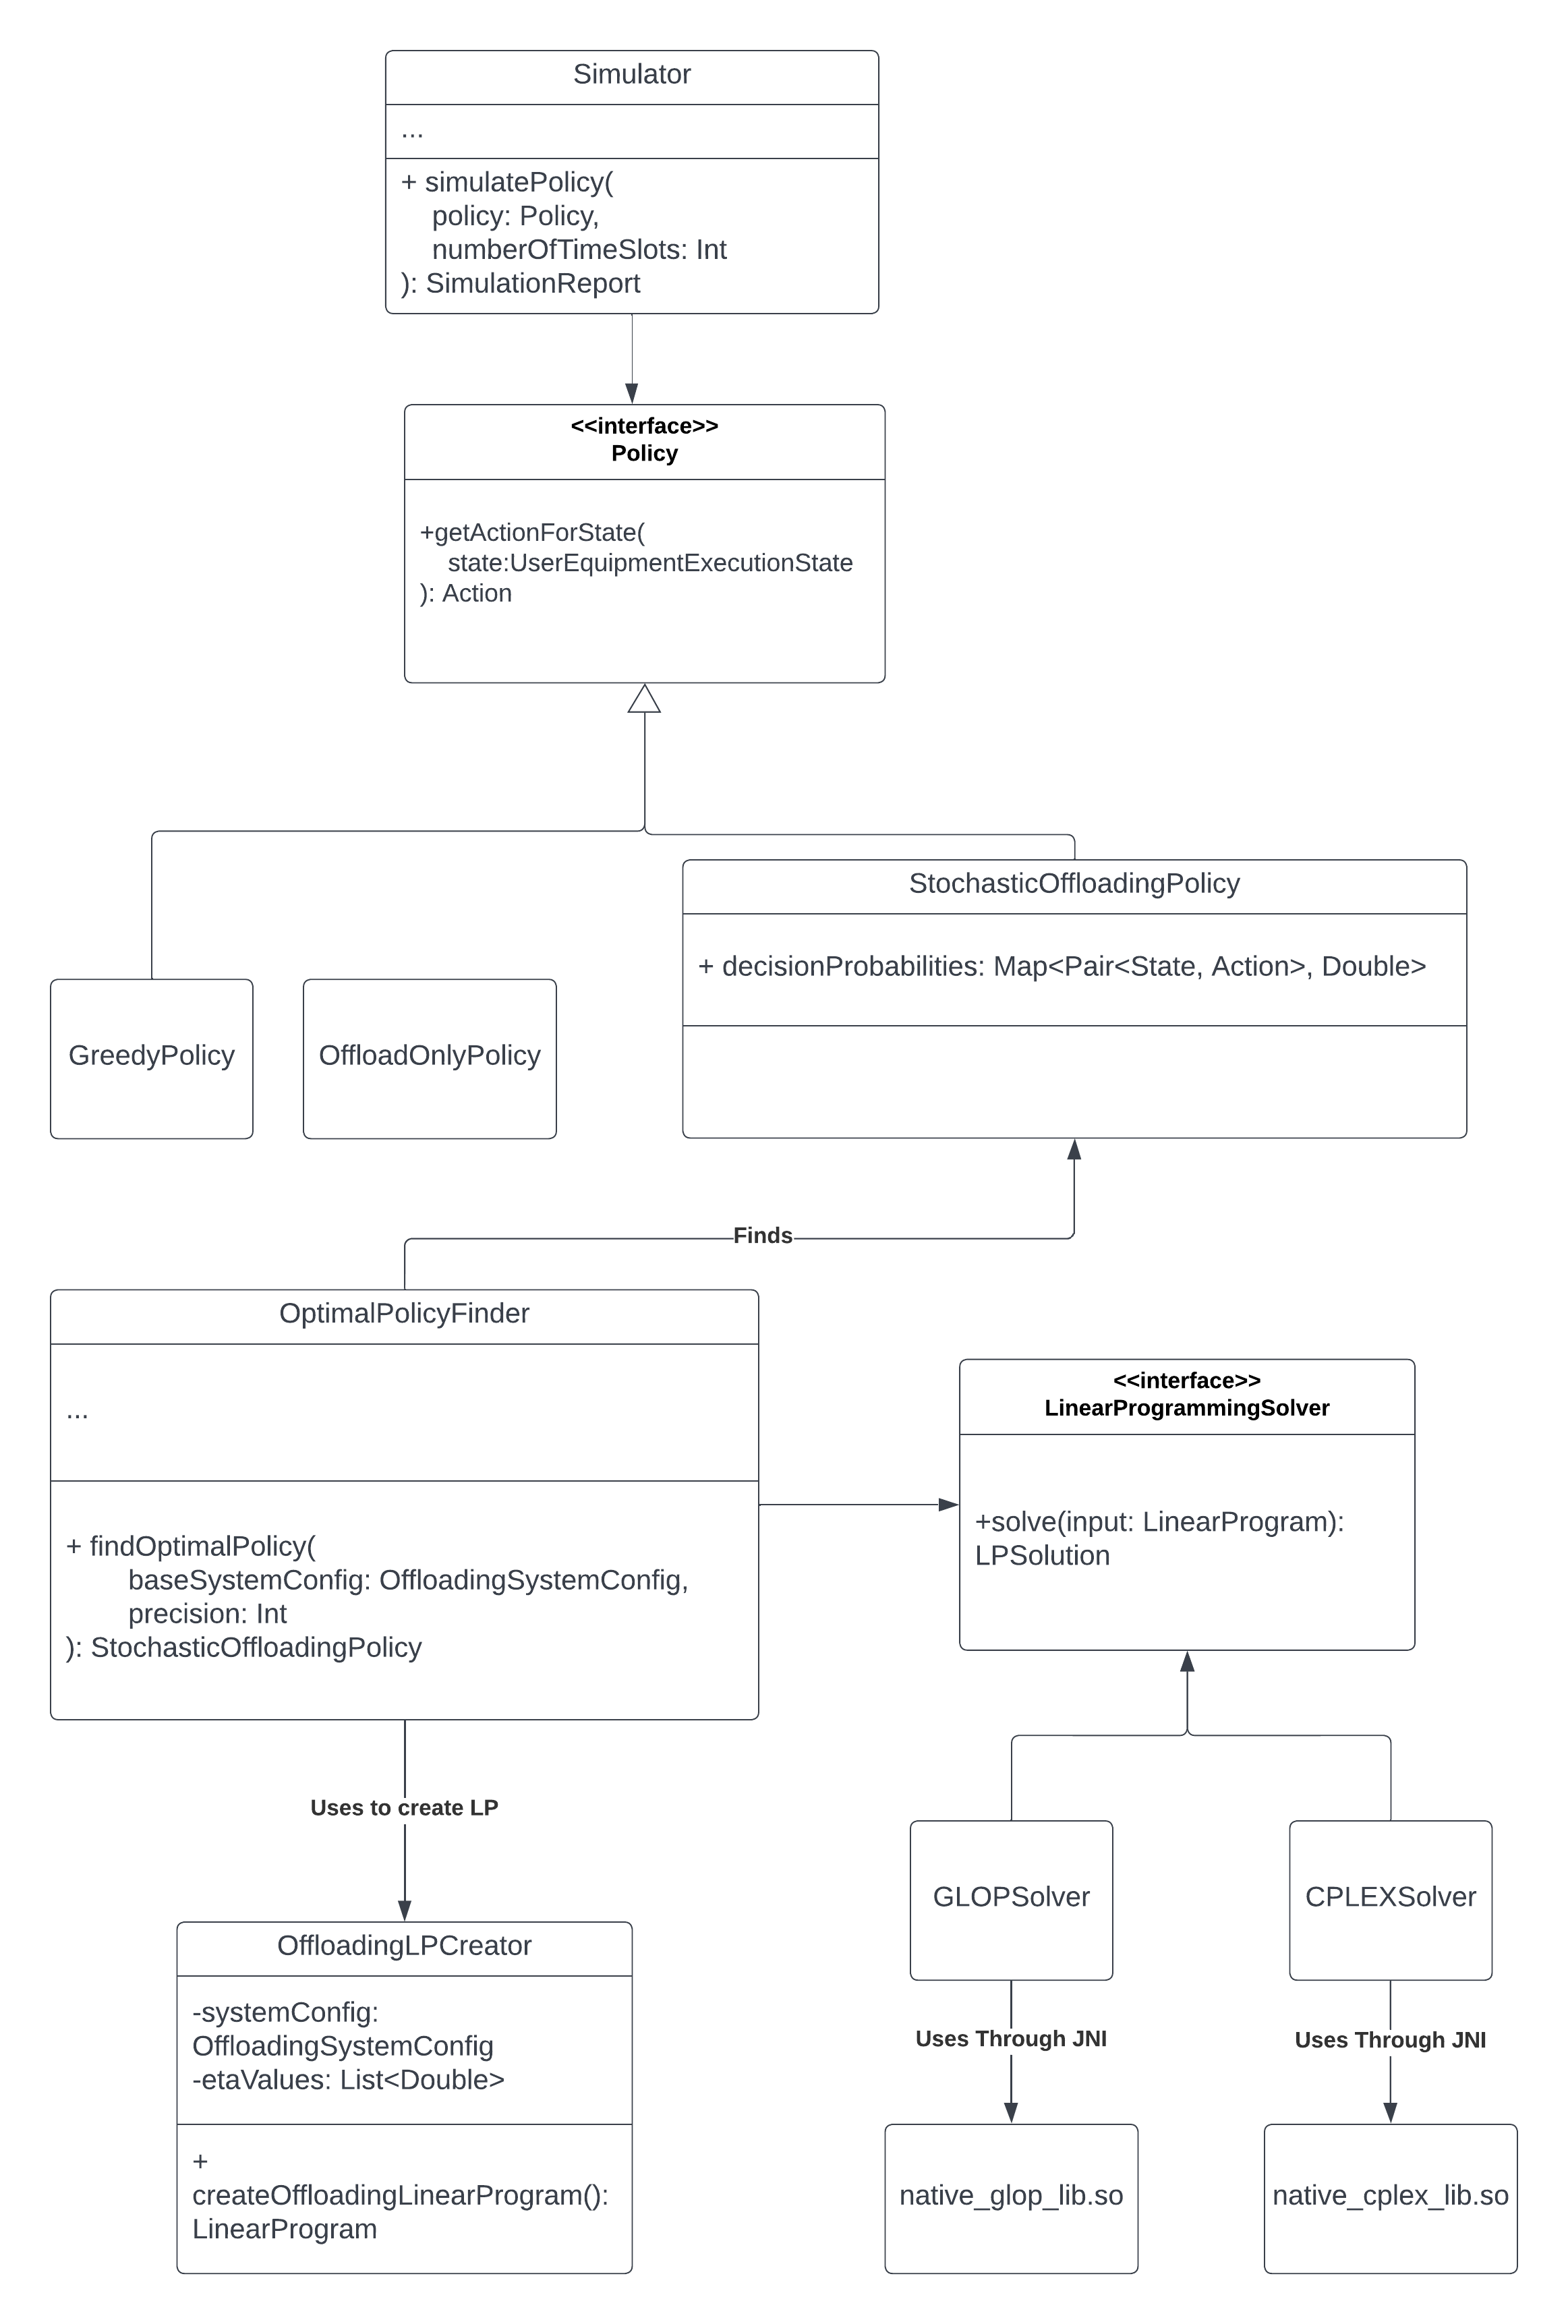
\includegraphics[width=0.9\textwidth]{cdiagram.png}
	\caption{کلاس دیاگرام فریم‌ورک \lr{Kompute}}
\end{figure}
\newpage
\subsection{ساخت و حل یک مسئله تخلیه وظیفه نمونه در \lr{Kompute}}
در کد نمونه زیر مسئله تخلیه وظیفه‌ برای محیط پردازش لبه‌ای با دو صف\footnote{شرایط بر اساس تقسیم‌بندی وظایف به \lr{Heavy} و \lr{Light} در اینترنت اشیا} حل شده است.
\begin{latin}
\begin{lstlisting}[language=Kotlin]
fun main(args: Array<String>) {
	val systemConfig = OffloadingSystemConfig(
		userEquipmentConfig = UserEquipmentConfig(
			stateConfig = UserEquipmentStateConfig(
				taskQueueCapacity = 5,
				tuNumberOfPackets = listOf(1, 3),
				cpuNumberOfSections = listOf(7, 2),
				numberOfQueues = 2
			),
			componentsConfig = UserEquipmentComponentsConfig(
				alpha = listOf(0.4, 0.9),
				beta = 0.90,
				etaConfig = null,
				pTx = 1.0,
				pLocal = 0.8,
				pMax = 1.7
			)
		),
		environmentParameters = EnvironmentParameters(
			nCloud = listOf(1, 1),
			tRx = 0.5,
		)
	)
	
	val optimalPolicy = RangedOptimalPolicyFinder.findOptimalPolicy(
		baseSystemConfig = systemConfig, 
		precision = 10
	)
	/*
	// For multi-threaded execution use this instead:
	
	val optimalPolicy = ConcurrentRangedOptimalPolicyFinder(
		baseSystemConfig = systemConfig
	).findOptimalPolicy(precision = 10, numberOfThreads = 8)
	*/
	
	
	val decisionProbabilities: Map<StateAction, Double>
	= optimalPolicy.stochasticPolicyConfig.decisionProbabilities
	
	println(decisionProbabilities)
}
\end{lstlisting}
\end{latin}
\newpage
\section{نتایج شبیه‌سازی}
در این بخش عملکرد استراتژی یافت شده توسط الگوریتم بخش قبل را با چهار الگوریتم پایه زیر مقایسه می‌کنیم:
\begin{enumerate}
	\item استراتژی فقط تخلیه\LTRfootnote{Offload Only} که همه‌ی وظایف را تخلیه می‌کند
	\item استراتژی حریصانه، تخلیه اول\LTRfootnote{Greedy (Offload First)} که در هر بازه زمانی اگر واحد ارسال یا پردازنده بیکار باشند به هر کدام از آنها یک وظیفه از صفی رندوم تخصیص می‌دهد و در صورتی که تنها یک وظیفه در صف باشد و مجبور به انتخاب بین تخلیه و اجرای محلی باشد، تخلیه را انتخاب می‌کند.
	\item استراتژی حریصانه، محلی اول\LTRfootnote{Greedy (Local First)} که در هر بازه زمانی اگر واحد ارسال یا پردازنده بیکار باشند به هر کدام از آنها یک وظیفه از صفی رندوم تخصیص می‌دهد و در صورتی که تنها یک وظیفه در صف باشد و مجبور به انتخاب بین تخلیه و اجرای محلی باشد، اجرای محلی را انتخاب می‌کند.
	\item استراتژی فقط (اجرای) محلی\LTRfootnote{Local Only}
\end{enumerate}
\newpage
\subsection{شبیه‌سازی تک صف}
با توجه به اینکه روش ارائه شده توسط ما حالت گسترش یافته \cite{Liu} است، ابتدا محیط تست ارائه شده در آن پژوهش را برای تست الگوریتم در نظر می‌گیریم. پارامترهای این محیط در جدول \ref{table:parameters-singlequeue} خلاصه شده اند. نتیجه این آزمایش در شکل \ref{plot:singleQueue} مشاهده می‌شود.

% Please add the following required packages to your document preamble:
\begin{table}[H]
	\centering
	\begin{tabular}{@{}lllllllll@{}}
		\toprule
		\textbf{پارامتر} & $P_1$ & $L_1$ & $\beta$ & $P_{tx}$ & $P_{loc}$ & $P_{max}$ & $C_1$ & $t_{rx}$ \\ \midrule
		مقدار             & 1    & 17   & 0.4  & 1.0 & 0.8  & 1.6  & 1    & 0.0   \\ \bottomrule
	\end{tabular}
	\caption{پارامترهای محیط پردازش لبه‌ای در سناریو تک صف}
	\label{table:parameters-singlequeue}
\end{table}

\begin{figure}[H]
	\centering
	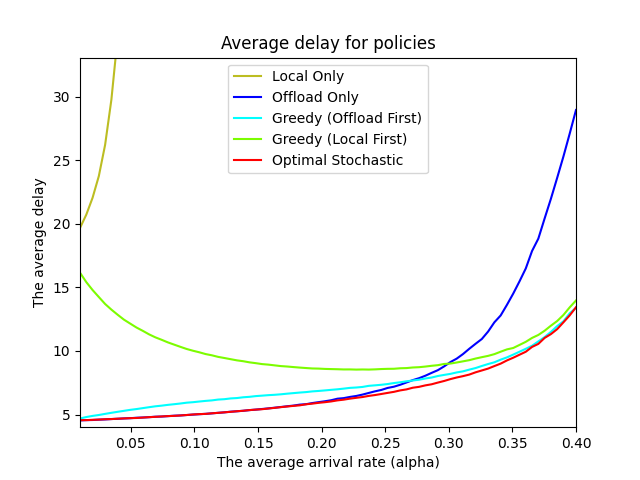
\includegraphics[width=0.7\textwidth]{PlotLiuLimitedSingleQueue.png}
	\caption{تاخیر سرویس به ازای نرخ ورود در حالت تک صف}
	\label{plot:singleQueue}
\end{figure}
همانطور که مشاهده می‌شود استراتژی تخلیه تصادفی یافت شده از تمام الگوریتم‌های پایه بهتر عمل می‌کند و شکل منحنی‌های نمودار با \cite{Liu} مطابقت دارد.
\newpage
\subsubsection{شبیه‌سازی دو صف با یک صف ثابت}
در این قسمت سناریوی تست به این گونه است که به ازای مقادیر مختلف نرخ ورود برای صف شماره یک و مقدار ثابت صف شماره دو مشاهده می‌شود.
\begin{figure}[H]
	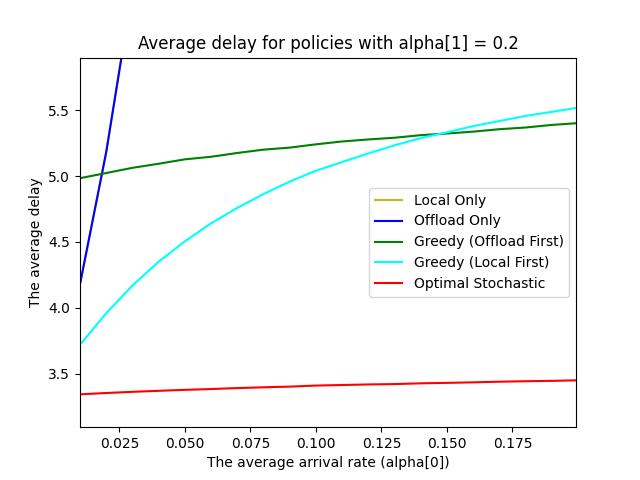
\includegraphics[width=\textwidth]{FixedRanged.png}
\end{figure}
\newpage
\subsubsection{شبیه‌سازی دو صف متغیر}
\begin{figure}[H]
	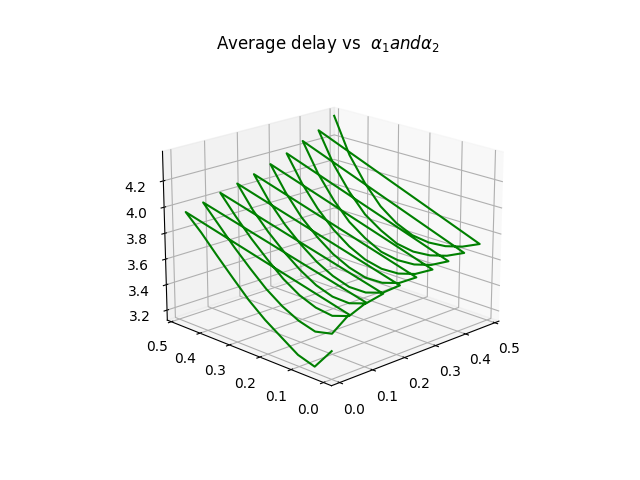
\includegraphics[width=\textwidth]{Plot3d.png}
\end{figure}
\newpage
\subsubsection{تست کارآمدی}
\begin{table}[H]
	\centering
	\begin{latin}		
		\resizebox{\textwidth}{!}{
		\begin{tabular}{llllll}
			\hline
			\textbf{Policy} & Optimal & Local Only & Greedy (Local First) & Greedy (Offload First) & Offload Only \\ \hline
			Value           & 100.0   & 23.33      & 72.49                & 92.95                  & 74.62        \\ \hline
		\end{tabular}
	}
	\end{latin}
\end{table}
\clearpage
